%
% File udst2018.tex

\documentclass[11pt,a4paper]{article}
\usepackage[hyperref]{udst2018}
\usepackage{times}
\usepackage{latexsym}
\usepackage{amsmath}
\usepackage{tikz}
\usepackage{tikz-dependency}
\usepackage[warn]{textcomp}
\usepackage[font=small]{caption}
\usepackage{subcaption}
\usepackage{multirow}
\usepackage{url}
\usepackage{etoolbox}
\usepackage{xr}

\newcommand{\com}[1]{}
\newcommand{\oa}[1]{\footnote{\color{red}OA: #1}}
\newcommand{\daniel}[1]{\footnote{\color{blue}Daniel: #1}}


\hyphenation{SemEval}

\DeclareMathOperator*{\argmin}{argmin}
\DeclareMathOperator*{\argmax}{argmax}

\makeatletter
\patchcmd\@combinedblfloats{\box\@outputbox}{\unvbox\@outputbox}{}{%
   \errmessage{\noexpand\@combinedblfloats could not be patched}%
}%
 \makeatother


\usetikzlibrary{shapes,shapes.misc}


\aclfinalcopy 
\def\aclpaperid{***} %  Enter the Paper ID here for final camera ready copy

%\setlength\titlebox{5cm}
% You can expand the titlebox if you need extra space
% to show all the authors. Please do not make the titlebox
% smaller than 5cm (the original size); we will check this
% in the camera-ready version and ask you to change it back.

\title{TUPA: the HUJI System for the CoNLL 2018 UD Shared Task}
% Applying a Transition-Based General DAG Parser to Universal Dependencies

\author{Daniel Hershcovich$^{1,2}$ \\
  \\\And
  Omri Abend$^2$ \\
  $^1$The Edmond and Lily Safra Center for Brain Sciences \\
  $^2$School of Computer Science and Engineering \\
  Hebrew University of Jerusalem \\
  \texttt{\{danielh,oabend,arir\}@cs.huji.ac.il}
  \\\And
  Ari Rappoport$^2$
}

\date{}

\begin{document}
\maketitle
\begin{abstract}
  We apply TUPA, a transition-based parser
  designed for parsing UCCA (a cross-linguistic
  semantic annotation scheme),
  to Universal Dependency Parsing.
  By employing a conversion protocol for representing
  UD trees and graphs in a UCCA-like unified DAG format,
  we train TUPA without modification on the UD
  parsing task.
\end{abstract}

\section{Introduction}\label{sec:introduction}




\begin{figure}[ht]
\begin{subfigure}{0.47\textwidth}
  \centering
    \begin{dependency}[text only label, label style={above}, font=\small]
    \begin{deptext}[column sep=.8em,ampersand replacement=\^]
    After \^ graduation \^ , \^ John \^ moved \^ to \^ Paris \\
    \end{deptext}
        \depedge[edge unit distance=1ex]{2}{1}{case}
        \depedge[edge unit distance=1ex]{4}{3}{punct}
        \depedge[edge unit distance=1ex]{5}{4}{nsubj}
        \depedge[edge unit distance=1ex, edge end x offset=-2pt]{2}{5}{obl}
        \depedge[edge unit distance=1ex]{7}{6}{case}
        \deproot[edge unit distance=1.5ex]{5}{root}
        \depedge[edge unit distance=1.5ex]{5}{7}{obl}
    \end{dependency}
  \caption{\label{fig:original_examples}Example UD tree.
  %Each word has exactly one head, and there is a single root.
  Edge labels express syntactic relations.}
\end{subfigure}
\begin{subfigure}{0.47\textwidth}
  \centering
  \scalebox{.95}{
  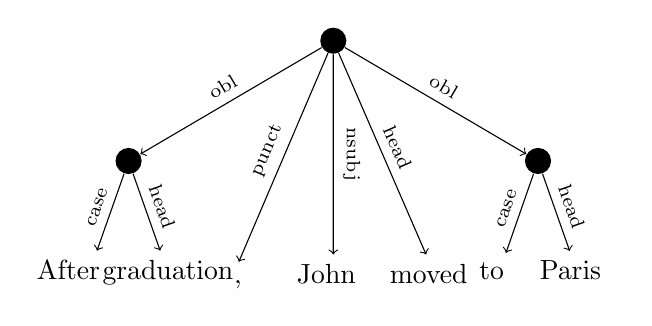
\begin{tikzpicture}[level distance=17mm, ->,
      every node/.append style={sloped,anchor=south,auto=false,font=\scriptsize},
      level 1/.style={sibling distance=13mm},
      level 2/.style={sibling distance=1cm}]
    \tikzstyle{word} = [font=\rmfamily,color=black]
    \node (ROOT) [fill=black,circle] {}
      child {node (after) [fill=black,circle] {}
      {
        child {node [word] {After{\color{white}g}\quad\quad} edge from parent node {case}}
        child {node [word] {\quad graduation\quad\quad} edge from parent node {head}}
      } edge from parent node {obl}}
      child {node {}
      {
        child {node [word] (comma) {\quad,{\color{white}g}} edge from parent [draw=none]}
      } edge from parent [draw=none]}
      child {node {}
      {
        child {node [word] (John) {John{\color{white}g}} edge from parent [draw=none]}
      } edge from parent [draw=none]}
      child {node {}
      {
        child {node [word] (moved) {moved{\color{white}g}} edge from parent [draw=none]}
      } edge from parent [draw=none]}
      child {node (to) [fill=black,circle] {}
      {
          child {node [word] {to{\color{white}g}} edge from parent node {case}}
          child {node [word] {Paris{\color{white}g}} edge from parent node {head}}
      } edge from parent node {obl}}
      ;
      \draw (ROOT) to node {punct} (comma);
      \draw (ROOT) to node {nsubj} (John);
      \draw (ROOT) to node {head} (moved);
  \end{tikzpicture}}
  \captionof{figure}{UD}\label{fig:converted_example_ud}
\end{subfigure}

\caption{Graph after conversion to  the unified DAG format
(with pre-terminals omitted: each terminal drawn in place of its parent).
Figure~\ref{fig:converted_example_ud} presents a converted UD graph.
Intermediate non-terminals and \textit{head} edges are introduced.
While converted UD graphs form trees, enhanced++ UD graphs may not.}\label{fig:converted_examples}
\end{figure}


%%%%%%%%%%%%%%%%%%%%%%%%%%%%%%%%%%%%%%%%%%%%%%%%%%%%%%%%%%%%%%%%%%%%%%%%%%%%%%%%%%%%%%%%
\section{Unified DAG Format}\label{sec:format}

To apply our parser to UD,
we convert it into a unified DAG format, which is inclusive enough to
allow representing any of the schemes with very little loss of information.\footnote{See
Supplementary Material for more conversion details.}

The format consists of a rooted DAG, where the tokens are the terminal nodes.
As in the UCCA format, edges are labeled (but not nodes),
and are divided into \textit{primary} and \textit{remote} edges,
where the primary edges form a tree (all nodes have at most one primary parent,
and the root has none).
Remote edges enable reentrancy, and thus together with primary edges
form a DAG.
Figure~\ref{fig:converted_examples} shows examples for converted graphs.

\paragraph{Converting bilexical dependencies.}
To convert UD into the unified DAG format,
we add a pre-terminal for each token,
and attach the pre-terminals according to the original dependency edges:
traversing the tree from the root down, for each head token we create a non-terminal
parent with the edge label {\it head},
and add the node's dependents as children of the created non-terminal node
(see Figure~\ref{fig:converted_example_ud}).


%%%%%%%%%%%%%%%%%%%%%%%%%%%%%%%%%%%%%%%%%%%%%%%%%%%%%%%%%%%%%%%%%%%%%%%%%%%%%%%%%%%%%%%%
\section{General Transition-based DAG Parser}\label{sec:model}

We extend TUPA \cite{hershcovich2017a}, 
a transition-based parser 
originally developed for UCCA,  to support UD parsing.

First used for projective syntactic dependency tree parsing \cite{Nivre03anefficient},
transition-based parsers have since been generalized to parse into many other
graph families, such as (discontinuous) constituency trees \cite[e.g., ][]{zhang2009transition,maier-lichte:2016:DiscoNLP},
and DAGs \cite[e.g.,][]{sagae2008shift,du-EtAl:2015:SemEval}. %ribeyre-villemontedelaclergerie-seddah:2014:SemEval,
Transition-based parsers apply \textit{transitions}
incrementally to an internal state defined by a buffer $B$ of remaining tokens 
and nodes, a stack $S$ of unresolved nodes, and a labeled graph $G$ of 
constructed nodes and edges.
When a terminal state is reached, the graph $G$ is the final output.
A classifier is used at each step to select the next transition, 
based on features that encode the current state.
%During training, an oracle converts the gold-standard annotations into
% training instances.




\subsection{TUPA's Transition Set}\label{sec:transition_set}

Given a sequence of tokens $w_1, \ldots, w_n$,
we predict a rooted graph $G$ whose terminals are the tokens.
Parsing starts with the root node on the stack,
and the input tokens in the buffer.

The TUPA transition set includes
the standard \textsc{Shift} and \textsc{Reduce} operations,
\textsc{Node$_X$} for creating a new non-terminal node and an $X$-labeled edge,
\textsc{Left-Edge$_X$} and \textsc{Right-Edge$_X$} to create a new primary $X$-labeled edge,
\textsc{Left-Remote$_X$} and \textsc{Right-Remote$_X$} to create a new remote $X$-labeled edge,
\textsc{Swap} to handle discontinuous nodes,
and \textsc{Finish} to mark the state as terminal.

Although UCCA contains nodes without any text tokens as descendants
(called \textit{implicit units}),
these nodes are infrequent and only cover 0.5\% of non-terminal nodes.
For this reason we follow previous work \cite{hershcovich2017a} and discard implicit units from
the training and evaluation,
and so do not include transitions for creating them.

In AMR, implicit units are considerably more common, as any unaligned concept
with no aligned descendents is implicit (about 6\% of the nodes).
Implicit AMR nodes usually result from alignment errors, or from abstract concepts
which have no explicit realization in the text \cite{buys2017oxford}.
We ignore implicit nodes when training on AMR as well.
TUPA also does not support node labels, 
which are ubiquitous in AMR but absent in UCCA structures (only edges are labeled in UCCA). 
We therefore only produce edge labels and not node labels when training on AMR.

\begin{figure}[t]
   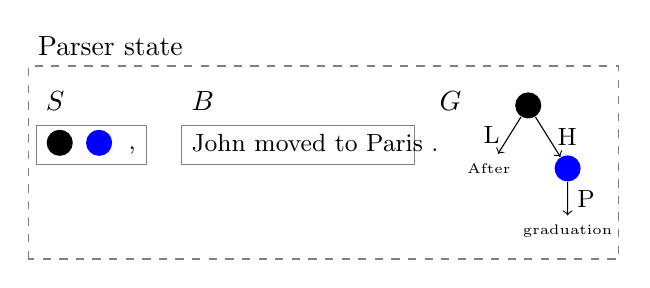
\begin{tikzpicture}[level distance=8mm, sibling distance=1cm]
   \node[anchor=west] at (0,1.5) {Parser state};
   \draw[color=gray,dashed] (0,-1.2) rectangle (7.5,1.25);
   \draw[color=gray] (.1,0) rectangle (1.5,.5);
   \node[anchor=west] at (.1,.8) {$S$};
   \node[fill=black, circle] at (.4,.275) {};
   \node[fill=blue, circle] at (.9,.275) {};
   \node[anchor=west] at (1.15,.175) {\small ,};
   \draw[color=gray] (1.95,0) rectangle (4.9,.5);
   \node[anchor=west] at (1.95,.8) {$B$};
   \node[anchor=west] at (1.95,.275) {\small John moved to Paris .};
   \node[anchor=west] at (5.1,.8) {$G$};
   \node[fill=black, circle] at (6.35,.75) {}
     child {node  {\tiny After} edge from parent [->] node[left] {\small L}}
     child {node [fill=blue, circle] {}
     {
       child {node {\tiny graduation} edge from parent [->] node[right] {\small P}}
     } edge from parent [->] node[right] {\small H} };
   \end{tikzpicture}
   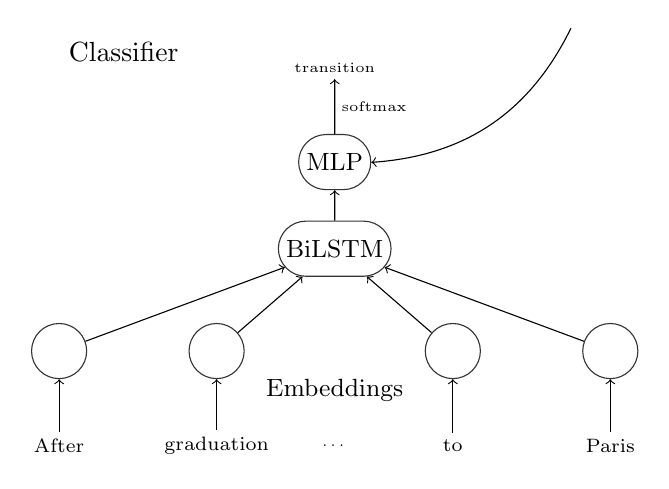
\begin{tikzpicture}[->]
   \node[anchor=west] at (0,6) {Classifier};
   \tiny
   \tikzstyle{main}=[rounded rectangle, minimum size=7mm, draw=black!80, node distance=12mm]
   \node[main] (specific) at (3.5,3.5) {\small BiLSTM};
   \node (embeddings) at (3.5,1.7) {\small Embeddings};
   \foreach \i/\word in {0/{After},2/{graduation},5/{to},7/{Paris}} {
       \node (x\i) at (\i,1) {\scriptsize \word};
       \node[main] (e\i) at (\i,2.2) {};
       \path (x\i) edge (e\i);
       \path (e\i) edge (specific);
   }
    \node (x4) at (3.5,1) {\ldots};
    \node[main] (mlp) at (3.5,4.6) {\small MLP};
    \path (specific) edge (mlp);
    \coordinate (state) at (6.5,6.3);
    \path (state) edge [bend left] (mlp);
    \node (transition) at (3.5,5.8) {transition};
    \path (mlp) edge node[right] {softmax} (transition);
   \end{tikzpicture}
\caption{Illustration of the TUPA model from \citet{hershcovich2018multitask}.
Top: parser state.
Bottom: BiLTSM architecture.}\label{fig:single_model}
\end{figure}


%%%%%%%%%%%%%%%%%%%%%%%%%%%%%%%%%%%%%%%%%%%%%%%%%%%%%%%%%%%%%%%%%%%%%%%%%%%%%%%%%
\subsection{Transition Classifier}\label{sec:classifier}

To predict the next transition at each step,
we use a BiLSTM with embeddings as inputs,
followed by an MLP and a softmax layer for classification \cite{kiperwasser2016simple}.
The model is illustrated in Figure~\ref{fig:single_model}.
Inference is performed greedily,
and training is done with an oracle that yields the set of all optimal 
transitions at a given state (those that lead to a state from which the gold graph is still reachable).
Out of this set, the actual transition performed in training is the one
with the highest score given by the classifier,
which is trained to maximize the sum of log-likelihoods of all 
optimal transitions at each step.




\paragraph{Features.}
We use the original TUPA features,
representing the words, POS tags, syntactic dependency relations, and previously predicted edge labels
for nodes in specific locations in the parser state.
In addition, for each token
we use embeddings representing the one-character prefix, three-character suffix,
shape (capturing orthographic features, e.g., ``Xxxx''),
and named entity type,\footnote{See Supplementary Material for a full listing of features.}
all provided by spaCy \cite{spacy2}.\footnote{\url{http://spacy.io}}
To the learned word vectors, we concatenate the 250K most frequent word vectors from fastText
\cite{bojanowski2016enriching},\footnote{\url{http://fasttext.cc}}
pre-trained over Wikipedia and updated during training.
%For AMR we add node label features according to gold node labels.


\paragraph{Constraints.}
As each annotation scheme has different constraints on the allowed graph structures,
we apply these constraints separately for each task.
During training and parsing, the relevant constraint set rules out some of the transitions
according to the parser state.
Some constraints are task-specific, others are generic.
For example, in UCCA, a terminal may only have one parent.
In AMR, a concept corresponding to a PropBank frame may only have 
the core arguments defined for the frame as children.
An example of a generic constraint is that stack nodes 
that have been swapped
should not be swapped again \cite{hershcovich2018multitask}.


\section{Training details}\label{sec:details}

\paragraph{Training.}

The model is implemented using DyNet \cite{neubig2017dynet}.\footnote{\url{http://dynet.io}}


\begin{table}[h]
\centering
\small
\setlength\tabcolsep{2pt}
\begin{tabular}{l|c|ccccc}
&& \multicolumn{3}{c}{\bf Multitask} \\ 
\bf Hyperparameter &  \bf Single & \bf Main & \bf Aux & \bf Shared \\
\hline
Pre-trained word dim. & 300 &&& 300 \\
Learned word dim. & 200 &&& 200 \\
POS tag dim. & 20 &&& 20 \\
Dependency relation dim. & 10 &&& 10 \\
Named entity dim. & 3 &&& 3 \\
Punctuation dim. & 1 &&& 1 \\
Action dim. & 3 &&& 3 \\
Edge label dim. & 20 & 20 \\
\hline
MLP layers & 2 & 2 & 1 \\
MLP dimensions & 50 & 50 & 50 \\
BiLSTM layers & 2 & 2 & & 2 \\
BiLSTM dimensions & 500 & 300 & & 300
\end{tabular}
\caption{Hyperparameter settings.
Middle column shows hyperparameters used for the single-task architecture,
described in \S\ref{sec:classifier}, and
right column for the multitask architecture,
described in \S\ref{sec:multitask}.
\textbf{Main} refers to parameters specific to the main task---UCCA parsing
(task-specific MLP and BiLSTM, and edge label embedding),
\textbf{Aux} to parameters specific to each auxiliary task
(task-specific MLP, but no edge label embedding since the tasks are unlabeled),
and \textbf{Shared} to parameters shared among all tasks
(shared BiLSTM and embeddings).\label{tab:hyperparams}}
\end{table}


\paragraph{Hyperparameters.}

We initialize embeddings randomly.
We use dropout \cite{srivastava2014dropout} between MLP layers, and recurrent dropout
\cite{NIPS2016_6241} between BiLSTM layers, both with $p=0.4$.
We also use word ($\alpha=0.2$), tag ($\alpha=0.2$) and dependency relation ($\alpha=0.5$) dropout
\cite{kiperwasser2016simple}.\footnote{In training, the embedding for a feature value $w$ is
replaced with a zero vector with a probability of $\frac{\alpha}{\#(w)+\alpha}$,
where $\#(w)$ is the number of occurrences of $w$ observed.}
In addition, we use a novel form of dropout, \textit{node dropout}:
with a probability of 0.1 at each step, all features associated with a single
node in the parser state are replaced with zero vectors.
For optimization we use a minibatch size of 100, decaying all weights by $10^{-5}$ at each update,
and train with stochastic gradient descent for $N$ epochs with a learning
rate of 0.1, followed by AMSGrad \cite{j.2018on} for $N$ epochs with
$\alpha=0.001,\beta_1=0.9$ and $\beta_2=0.999$.
We use $N=50$ for English and German, and $N=400$ for French.
We found this training strategy better than using only one of the optimization methods,
similar to findings by \citet{keskar2017improving}.
We select the epoch with the best average labeled $F_1$ score on the
UCCA development set.
Other hyperparameter settings are listed in Table~\ref{tab:hyperparams}.


\paragraph{Evaluation.}

We evaluate on UCCA using labeled precision, recall and $F_1$ 
on primary and remote edges,
following previous work \cite{hershcovich2017a}.
Edges in predicted and gold graphs are matched by terminal yield and label.
Significance testing of improvements over the single-task model is done
by the bootstrap test \cite{berg2012empirical}, with $p<0.05$.

%\subsection{Ensembling}
%
%During inference, we use Product of Experts \cite[PoE; ][]{hinton2002training} to combine the predictions
%of three models trained in the same setting, but with different random seeds. The transition selected is
%\[
%\argmax_{t\in T}\sum_{i=1}^3\big[\log(\mathrm{softmax}(m_i(s)))\big]_t
%\]
%where $T$ is the set of possible transitions, $m_i$ are the combined models, and $s$ is the current state.
%
%In order to ensemble multitask models, we combine models trained with the same auxiliary task.
%Another alternative is to combine models trained with different auxiliary tasks.\oa{don't write about alternatives,
%but rather on what we actually do}
%This provides greater variability between the combined models.



\section{Results}\label{sec:results}


Table~\ref{tab:id_results} presents our results.


\section{Conclusion}\label{sec:conclusion}

We demonstrate that semantic parsers can leverage a range of 
semantically and syntactically annotated data, to improve their performance.
Our experiments show that MTL improves UCCA parsing,
using AMR, DM and UD parsing as auxiliaries.
We propose a unified DAG representation, 
construct protocols for converting these schemes into the unified format,
and generalize a transition-based DAG parser to support all these tasks,
allowing it to be jointly trained on them.
%While the machine learning techniques we use are not novel,
%our contribution is in allowing these models to learn from
%significantly different tasks.

%A natural question is whether our method can benefit AMR, DM or UD parsing.
While we focus on UCCA in this work, our parser is capable of parsing any
scheme that can be represented in the unified DAG format,
and preliminary results on AMR, DM and UD are promising (see~\S\ref{sec:discussion}).
Future work will investigate whether a single
algorithm and architecture can be competitive on all of these parsing tasks,
an important step towards a joint many-task model for semantic parsing.



\bibliography{references}
\bibliographystyle{acl_natbib}

\end{document}

